\section{Activity: Vibrating Scale}
\subsection{Materials required}
\begin{enumerate}
    \item Scale
\item Desk or table
\end{enumerate}
\subsection{Procedure}
Place the scale on the desk so that about one-third of it is over the edge. Hold the part on the desk firmly with one hand. Push the free end of the scale downward. Release it quickly.
\begin{marginfigure}[-20\baselineskip]
  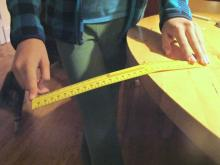
\includegraphics{scale-down}
  \caption[Sound with a scale]{Step 1. Push the free end of the scale downwards.}
\end{marginfigure}
\marginnote{\footnotesize Image credit: Ingrid Sulston, licensed under CC BY-NC-SA 4.0}
\begin{marginfigure}
  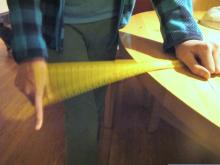
\includegraphics{scale-vibrate}
  \caption[Sound with a scale]{Step 2. Let the pushed end go.}
\end{marginfigure}
\marginnote{\footnotesize Image credit: Ingrid Sulston, licensed under CC BY-NC-SA 4.0}
\newthought{Observe} the movement of the scale. Do you hear a sound? Do you see the scale move up and down rapidly? What type of motion is this?